%%%%%%%%%%%%%%%%%%%%%%%%%%%%%%%%%%%%%%%%%
% a0poster Portrait Poster
% LaTeX Template
% Version 1.0 (22/06/13)
%
% The a0poster class was created by:
% Gerlinde Kettl and Matthias Weiser (tex@kettl.de)
% 
% This template has been downloaded from:
% http://www.LaTeXTemplates.com
%
% License:
% CC BY-NC-SA 3.0 (http://creativecommons.org/licenses/by-nc-sa/3.0/)
%
%%%%%%%%%%%%%%%%%%%%%%%%%%%%%%%%%%%%%%%%%

%----------------------------------------------------------------------------------------
%	PACKAGES AND OTHER DOCUMENT CONFIGURATIONS
%----------------------------------------------------------------------------------------

\documentclass[a0,portrait]{a0poster}

\usepackage[portuguese]{babel}%Formata as entradas para PT-BR
%\usepackage[utf8]{inputenc}
%\usepackage{verbatim}
\usepackage[document]{ragged2e}
\usepackage{multicol} % This is so we can have multiple columns of text side-by-side
\columnsep=100pt % This is the amount of white space between the columns in the poster
\columnseprule=3pt % This is the thickness of the black line between the columns in the poster

\usepackage[svgnames]{xcolor} % Specify colors by their 'svgnames', for a full list of all colors available see here: http://www.latextemplates.com/svgnames-colors

\usepackage{times} % Use the times font
%\usepackage{palatino} % Uncomment to use the Palatino font
%\usepackage{varioref}
%\usepackage{hyperref}
%\usepackage{epsfig}
\usepackage{graphicx} % Required for including figs
\graphicspath{{figures/}} % Location of the graphics files
\usepackage{booktabs} % Top and bottom rules for table
\usepackage[font=small,labelfont=bf]{caption} % Required for specifying captions to tables and figures
\usepackage{amsfonts, amsmath, amsthm, amssymb} % For math fonts, symbols and environments
\usepackage{mathrsfs}
\usepackage{wrapfig} % Allows wrapping text around tables and figures
\usepackage{setspace}
\usepackage{float}

\DeclareMathOperator{\ulp}{ULP}

\begin{document}
\onehalfspacing
%----------------------------------------------------------------------------------------
%	POSTER HEADER 
%----------------------------------------------------------------------------------------

% The header is divided into two boxes:
% The first is 75% wide and houses the title, subtitle, names, university/organization and contact information
% The second is 25% wide and houses a logo for your university/organization or a photo of you
% The widths of these boxes can be easily edited to accommodate your content as you see fit

\vspace*{-7cm}
\begin{figure}[!htb]
  \begin{minipage}{0.65\textwidth}
    
\includegraphics[width=.85\linewidth]{figs/LogoCNMAC2025}
  \end{minipage}\hfill
  \begin{minipage}{0.40\textwidth}
    \hspace{12cm}
    
\includegraphics[width=.4\linewidth]{figs/Logo_CEFET-MG}%INCLUIR LOGO DA SUA UNIVERSIDADE, REMOVER PHANTOM
  \end{minipage}
\end{figure}

\vspace{.5cm}
\begin{minipage}[b]{1.0\linewidth} %default 0.75
  \begin{center}
    \Huge \textbf{Análise Visual de Erros de Ponto Flutuante e das Units of Last Place em Experimentos Computacionais}\\
    %\Huge\textit{An Exploration of Complexity}\\[2cm] % Subtitle
    \huge \textbf{Enzo Rocha Leite Diniz Ribas$^{1}$, D'Afonseca, L. A.$^{2}$, Rocha, L. M.$^{3}$}\\
    [0.5cm] % Author(s)
    \huge Centro Federal de Educação Tecnológica de Minas Gerais, MG, Brasil\\[0.4cm] % University/organization
    \Large \texttt{enzorochaleitedinizribas@gmail.com$^{1}$, luis.dafonseca@gmail.com$^{2}$, lucasmartinsrocha@gmail.com$^{3}$}\\
  \end{center}
\end{minipage}
%
\vspace{1cm} % A bit of extra whitespace between the header and poster content

%----------------------------------------------------------------------------------------

\begin{multicols}{2} % This is how many columns your poster will be broken into, a portrait poster is generally split into 2 columns

  \justify % Justify all text

  %----------------------------------------------------------------------------------------
  %	ABSTRACT
  %----------------------------------------------------------------------------------------

  %\color{Navy} % Navy color for the abstract

  %\begin{abstract}
  \section*{Resumo}
  \vspace{-1cm}
  % O RESUMO deve ser claro, sucinto e explicar o(s) objetivo(s) pretendido(s), procurando justificar sua import\^ancia, os principais procedimentos adotados, os resultados mais expressivos e conclus\~oes. Se recomenda que o RESUMO n\~ao contenha f\'ormulas, cita\c c\~oes e/ou refer\^encias bibliogr\'aficas.

  Este trabalho apresenta resultados de estudos realizados em um projeto de
  iniciação científica e tem como objetivo explorar graficamente alguns efeitos
  do cálculos realizados com ponto flutuante e das Unidades de Última Posição
  (ULP's). Para implementação dos códigos, e geração de gráficos, foi utilizado a
  linguagem Python, assim como suas diversas bibliotecas.

  \vspace{1cm}

  \hspace{-0,5cm}\textbf{Palavras-Chave:}
  % m\'aximo de cinco, separadas por ponto e v\'i­rgula (;), procurando n\~ao repetir palavras do t\'i­tulo, escritas em letras min\'usculas, organizadas em ordem alfab\'etica crescente.
  Erros Numéricos; IEEE 754; Métodos Numéricos; Cancelamento Catastrófico; Ponto
  Flutuante.
  %\end{abstract}

  %----------------------------------------------------------------------------------------
  %	Introdu\c c\~ao
  %----------------------------------------------------------------------------------------

  %\begin{abstract}
  \section*{Introdu\c c\~ao}
  \vspace{-1cm}
  % A introdu\c c\~ao tem como objetivo posicionar o leitor dentro do tema que est\'a sendo desenvolvido. Deve conter a delimita\c c\~ao do universo da pesquisa, problema, objetivos, justificativa, hip\'oteses, metodologia de trabalho e sua relev\^ancia. Evitar o uso de palavras e ideias repetidas. Seja objetivo e preciso em suas considera\c c\~oes, evitando que a introdu\c c\~ao do trabalho fique longa e cansativa.

  Frequentemente, computadores são utilizados para realizar cálculos numéricos
  repetitivos e de grande complexidade. Mesmo assim, computadores possuem uma
  limitação física para representar números reais.

  Um erro comum em SPF's é o da perda de significância, ou cancelamento
  catastrófico, que ocorre quando é realizada uma operação com dois números muito
  próximos ou de grandezas muito diferentes, resultando em um valor com menos
  dígitos significativos do que os números originais, devido ao alinhamento de
  mantissa. Um exemplo desse comportamento é observado na função $f(x) = x^{23} +
    1 - x^{23}$, que é igual a $1$. Porém, ao avaliar $f$ usando ponto flutuante,
  obtemos o gráfico da Figura~\ref{fig:erros1}, em que o valor correto é exibido
  apenas até $x$ próximo de $4,9$. A partir de aproximadamente $x = 5,1$, a
  função assume o valor zero. Isso ocorre, pois o valor $x^{23}$ é muito maior
  que $1$, o que resulta na perda de significância, produzindo $x^{23} + 1 =
    x^{23}$.

  Entre $4,9$ e $5,1$ observamos a ocorrência de uma oscilação caótica
  relacionada com o valor da $\ulp(x^{23})$, que é 2. Para realizar a soma
  $x^{23} + 1$, o SPF precisa representar os dois números na mesma potência.
  Porém, o valor do expoente necessário para representar $x^{23}$ está associado
  à uma ULP igual a 2, em que o número 1 não pode ser representado e precisa ser
  arredondado. Esse arredondamento faz com que $x^{23} + 1$ seja igual a $x^{23}$
  ou $x^{23} + 2$, produzindo a oscilação observada.

  \begin{figure}[H]
    \centering
    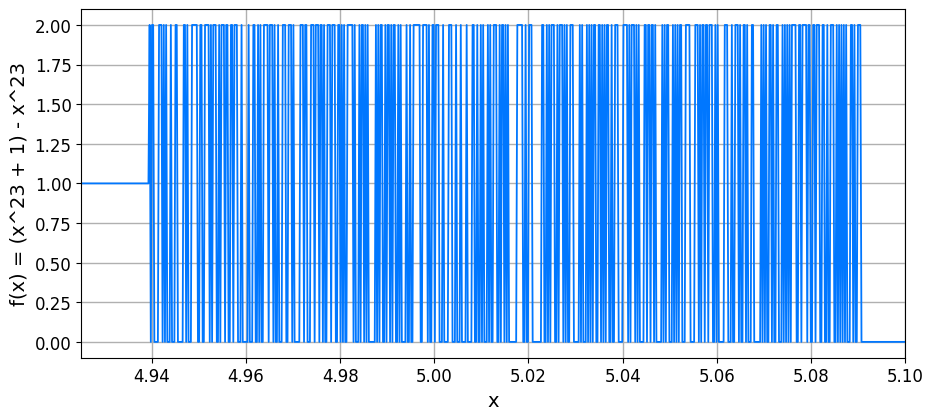
\includegraphics[width=.8\linewidth]{figs/erro1}
    \vspace{-.5cm}
    \caption{ {\small Resultado da avaliação da função $f(x) = x^{23} +
            1 - x^{23}$ num SPF IEEE de 64 \text{bits}. Fonte: Autor.}}
    \label{fig:erros1}
  \end{figure}
  %\end{abstract}

  %----------------------------------------------------------------------------------------
  %	OBJETIVOS
  %----------------------------------------------------------------------------------------

  %\color{Navy} % Navy color for the abstract

  %\begin{Objetivos}
  \section*{Objetivos}
  \vspace{-1cm}
  O objetivo geral deve resumir e apresentar a ideia central de um trabalho, descrevendo tamb\'em sua finalidade. Os objetivos espec\'i­ficos ir\~ao dar uma maior delimita\c c\~ao ao tema, al\'em de detalhar os processos necess\'arios para a realiza\c c\~ao do trabalho.

  %\end{Objetivos}

  %----------------------------------------------------------------------------------------
  %	Fundamenta\c c\~ao Te\'orica
  %----------------------------------------------------------------------------------------

  %\color{Navy} % Navy color for the abstract

  %\begin{Fundamenta\c c\~ao Te\'orica}
  \section*{Fundamenta\c c\~ao Te\'orica}
  \vspace{-1cm}
  % Apresenta as refer\^encias nas quais se baseia a pesquisa:\\
  % \begin{itemize}
  %   \item livros, artigos em revistas/peri\'odicos, teses de doutorado, disserta\c c\~oes
  %         de mestrado
  % \end{itemize}
  % O referencial te\'orico tem tamb\'em outras fun\c c\~oes:
  % \begin{itemize}
  %   \item permite que o autor tenha maior clareza,
  %   \item facilita a formula\c c\~ao de hip\'oteses e de suposi\c c\~oes,
  %   \item sinaliza para o m\'etodo mais adequado \`a solu\c c\~ao do problema,
  %   \item permite identificar qual o procedimento mais pertinente para a coleta e o
  %         tratamento dos dados, bem como o conte\'udo do procedimento escolhido.
  %   \item uma revis\~ao de literatura serve para verificar o que j\'a foi pesquisado do
  %         assunto.

  Um Sistema de Ponto Flutuante (SPF) é a maneira utilizada para aproximar
  números reais pelos computadores através de representações binárias compactas.
  Para a maioria dos computadores atuais, o padrão adotado é o definido pela
  IEEE-754~\cite{IEEE754}.

  Devido à natureza discreta e finita dos SPF's, erros de representação são
  intrínsecos e propagam-se em operações aritméticas sucessivas, se acumulando e
  podendo comprometer severamente a exatidão numérica do sistema.

  No padrão IEEE 754 um número de ponto flutuante é dividido em três partes. O
  primeiro bit, representa o \textbf{Sinal (S)} do número representado, indicando
  se o número é positivo (\( S = 0 \)) ou negativo (\( S = 1 \)); Os próximos $N$
  bits representão o \textbf{expoente (E)} com viés (bias), que é calculado como
  $\text{bias} = 2^{(N-1)} - 1$; E por fim, os últimos $M$ bits Representam a
  \textbf{Mantissa (M)} que é parte fracionária significativa do número.
  \begin{equation}
    x =
    \left(-1\right)^S
    \times
    \left(1.M\right)
    \times
    2^{E - \text{bias}},
    \label{eq:spf}
  \end{equation}
  Na mantissa, o termo $1.M$ indica que há um bit implícito ``1'' antes da mantissa nos números normalizados.

  A \textit{Unit of Last Place (ULP)} é a menor diferença entre dois números
  representáveis em ponto flutuante, ou seja, a distância entre um número e o
  próximo número representável~\cite{muller2005,kahan2004}. O conjunto de números
  se torna mais esparso quanto mais distante o número for de zero, aumentando o
  erro relativo. Dessa forma, a ULP se torna uma medida relativa importante para
  avaliar a precisão dos cálculos realizados com ponto flutuante, podendo ser
  calculada como
  \begin{equation}
    \ulp(x) = 2^{p - t + 1},
    \label{eq:ulp}
  \end{equation}
  em que $p$ é o expoente do número representado em ponto flutuante e $t$ é o número de bits da mantissa. A Figura~\ref{fig:ulp} mostra o gráfico da função $\ulp(x^{23})$ num SPF IEEE de 64 \text{bits}.

  \begin{figure}[h]
    \centering
    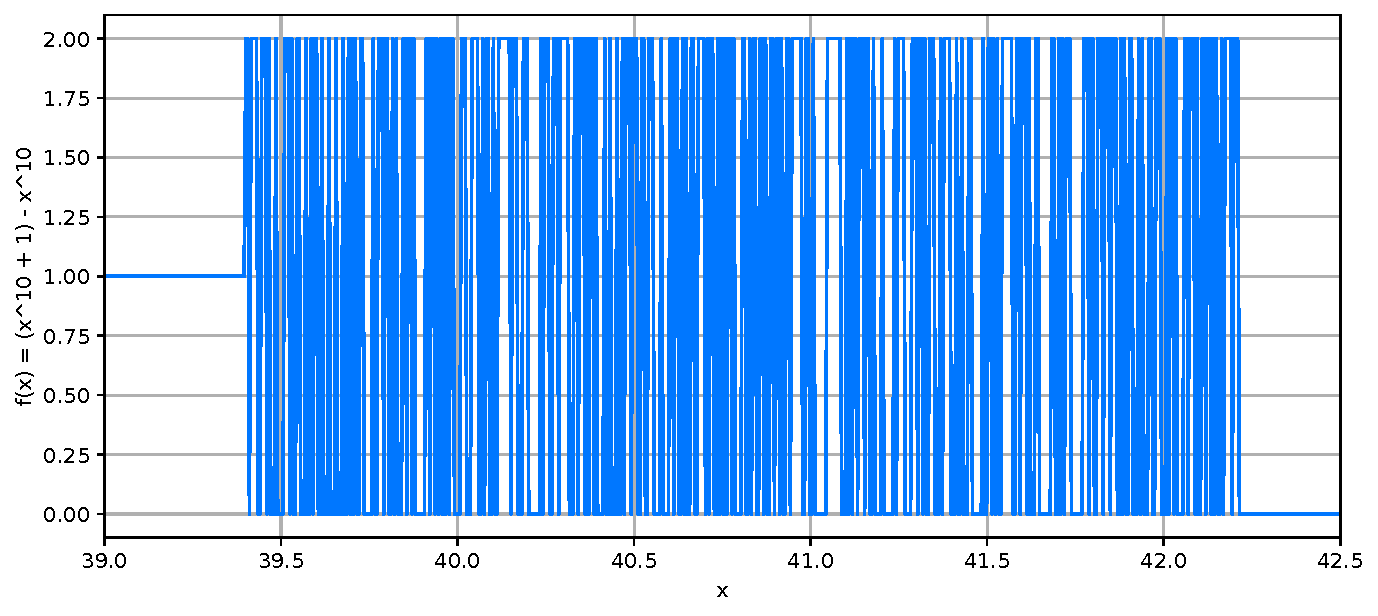
\includegraphics[width=.8\linewidth]{figs/NumError1_mplt.pdf}
    \vspace{-.5cm}
    \caption{ {\small Gráfico da Função $\ulp(x^{23})$ num SPF IEEE de 64 \text{bits}. Fonte: Autor.}}~\label{fig:ulp}
    \vspace{-.5cm}
  \end{figure}

  %\end{Fundamenta\c c\~ao Te\'orica}
  %----------------------------------------------------------------------------------------
  %	PROBLEM FORMULATION
  %----------------------------------------------------------------------------------------

  %\color{SaddleBrown} % SaddleBrown color for the introduction

  %\begin{center}
  \section*{Desenvolvimento e Metodologia ou Materiais e M\'etodos}
  %\end{center}
  %\begin{justify}
  %\setlength{\parindent}{5ex} \indent \par
  \vspace{-1cm}
  Descrever adequadamente o desenvolvimento e a metodologia utilizada para desenvolver o trabalho. Deve ser pertinente ao tema, procurando alcan\c car os objetivos j\'a apresentados.\\
  Caso use equa\c c\~oes, numerar descrevendo os par\^ametros.\\
  Figuras, tabelas e gr\'aficos devem ser apresentados com tamanho, qualidade e detalhes suficientes para a interpreta\c c\~ao e composi\c c\~ao gr\'afica final.
  Citar a fonte da ilustra\c c\~ao, tabela e gr\'afico e, caso seja do pr\'oprio autor, citar como ``Fonte: Elaborada pelo autor''.
  As legendas e fontes das figuras, tabelas e gr\'aficos devem ser escritos em fonte Times New Roman, tamanho 10 e o texto deve estar centralizado, em negrito e seguir o padr\~ao de numera\c c\~ao sucessivo ar\'abico. Centralizar as Figuras, Tabelas e Gr\'aficos.
  \textbf{Gr\'aficos e figuras:} devem apresentar-se sem bordas; a legenda deve ser posicionada logo abaixo da figura ou gr\'afico. Usar imagens coloridas se for necess\'ario destacar alguma informa\c c\~ao da Figura ou Gr\'afico.

  \textbf{Tabelas:} evitar tabelas extensas e dados sup\'erfluos; adequar seus tamanhos ao espa\c co \'util do papel e colocar, na medida do poss\'i­vel, apenas linhas cont\'i­nuas horizontais. As legendas devem ser autoexplicativas, localizadas abaixo da tabela, como no exemplo a seguir.

  \vspace{2cm}
  \begin{minipage}[b]{1.0\linewidth}
    \begin{center}
      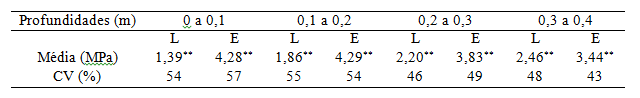
\includegraphics[width=37cm]{figs/tabela.png}
      \captionof{figure}{An\'alise do \'Indice de Cone (IC) nas linhas (L) e entrelinhas (E) de cana nas diferentes profundidades amostradas. Fonte: OLIVEIRA et al., 2008.}
    \end{center}
  \end{minipage}
  \vspace{-1cm}
  %\end{justify}

  %----------------------------------------------------------------------------------------
  %	NUMERICAL RESULTS 
  %----------------------------------------------------------------------------------------

  \section*{Resultados}
  \vspace{-1cm}
  Apresentar os resultados de maneira organizada e l\'ogica, fornecendo ao leitor as informa\c c\~oes mais representativas. \'E comum o uso de figuras e tabelas para ilustrar os dados apresentados de maneira a facilitar a compreens\~ao dos resultados obtidos. As legendas devem ser autoexplicativas, localizadas abaixo da tabela, como no exemplo a seguir.
  %\end{justify}

  %

  %\begin{wraptable}{l}{12cm} % Left or right alignment is specified in the first bracket, the width of the table %is in the second
  %\begin{tabular}{l l l}
  %\toprule
  %\textbf{Treatments} & \textbf{Response 1} & \textbf{Response 2}\\
  %\midrule
  %Treatment 1 & 0.0003262 & 0.562 \\
  %Treatment 2 & 0.0015681 & 0.910 \\
  %Treatment 3 & 0.0009271 & 0.296 \\
  %\bottomrule
  %\end{tabular}
  %\captionof{table}{\color{Green} Table caption}
  %\end{wraptable}

  %----------------------------------------------------------------------------------------
  %	CONCLUSIONS
  %----------------------------------------------------------------------------------------

  %\color{SaddleBrown} % SaddleBrown color for the conclusions to make them stand out

  \section*{Conclus\~oes}
  \vspace{-1cm}
  Devem basear-se, exclusivamente, nos resultados do trabalho. Ressaltar se os objetivos expostos inicialmente foram cumpridos e se a hip\'otese foi confirmada. Aspectos metodol\'ogicos tamb\'em devem ser abordados: dificuldades durante a pesquisa, resultados obtidos e qual o significado dos mesmos dentro da \'area de pesquisa. Quando poss\'i­vel, inserir outros tipos de estudos que poderiam ser feitos utilizando o mesmo tema e/ou outros aspectos a serem abordados a partir dos resultados apresentados.

  %\color{DarkSlateGray} % Set the color back to DarkSlateGray for the rest of the content

  %----------------------------------------------------------------------------------------
  %	REFERENCIAS
  %----------------------------------------------------------------------------------------
  \vspace{-1cm}
  \nocite{*} % Print all references regardless of whether they were cited in the poster or not
  \bibliographystyle{plain}
  \bibliography{refs}

  \section*{Agradecimentos (Opcional)}
  \vspace{-1cm}
  Inserir, ap\'os as conclus\~oes, de maneira sucinta os agradecimentos. Se o projeto for financiado por alguma ag\^encia de fomento, citar a fonte. Incluir a logomarca da sua universidade no lugar daquele modelo de logo no cabe\c calho.

  %----------------------------------------------------------------------------------------

\end{multicols}
\end{document}